\chapter{Proof of the Upper and Lower Bounds}
\myTop{The upper and lower bound of the \rubik{} will be presented and explained in this chapter. The upper bound needs to be proven, in order for it to be recognized. The lower bound is the bound which we want to find to state that any arbitrary \rubik{} can be solved in this number of twists. NEED REWRITE}

The lower bound is the number of twists required to solve the \rubik{} in the position which requires the most twists to solve.
The upper bound of the \rubik{} is the lowest number of twists needed to solve an arbitrary \rubik{} in the worst case scenario.
Proofs of the upper bound have been published several times, and it has been lowered each time.
A major breakthrough was when Thistlethwaite's algorithm was proven to be able to solve an arbitrary cube in 52 twists or less \cite{jaapthistle}.
Since then a lot of progress has been made in the field.
This section describes this progression.

\begin{figure}[ht]
	\centering
		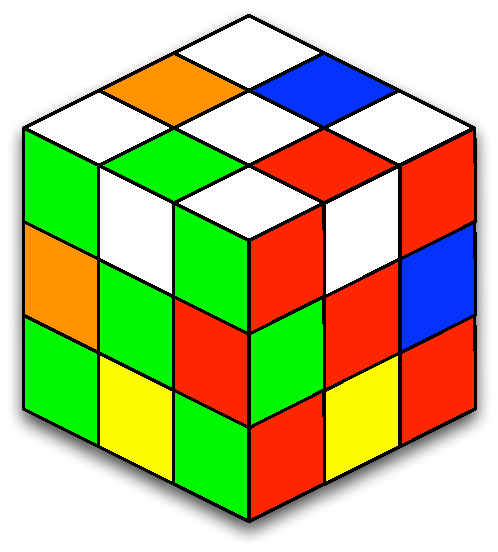
\includegraphics[scale = 0.7]{input/pics/superflip.pdf}
	\caption{\myCaption{The current upper and lower bound displayed on a graph. SKIFT BILLEDET FFS!!!!!!!!!!!!!!!!!!!!!!!!!!!!!!!!!!!!!!!!!!!!!!!!!!!!!!!!!!!!!!!!!!!!!!!}}
	\label{fig:superflip}
\end{figure}

\section{Set Solver}
\label{sec:setSolver}
The algorithm used to prove the current lowest upper bound is known as a set solver and uses Kociemba's algorithm. The set solver is a viable method for proving the upper bound because it does not solve every single cube but a whole set of cubes at the time as the name suggests. This means that it solves approximately 19.5 billion cubes at a time.
The set solver does this by finding all the move sequences of a relabeled cube of the distance $d$ that transforms the cube into \m{H}. 
The algorithm set solver is described in pseudo code below in algorithm \ref{alg:setSolver}.%All the move sequences to transform the unlabeled cube to $e$ is in a database so it is fast to find the shortest move sequence, once the move sequence to \m{H} has been found.

\begin{algorithm}[!h]                     
\caption{Set Solver \cite{rokicki09}}          
\label{alg:setSolver}        
\begin{algorithmic}[1]
\STATE {$f=\oslash$}
\STATE {$d=0$}
\WHILE {true} 
		\IF {$d \leq m$}
			\FOR {$b \in S^d$}
				\IF {$r(ab) = r(e)$}
					\STATE {$f = f \cup ab$}
				\ENDIF
			\ENDFOR
		\ENDIF
		\IF {$f = H$}
			\STATE {return $d$}
		\ENDIF
	\STATE {$d = d + 1$}
	\STATE {$f = f \cup fA$}
	\IF {$f = H$}
		\STATE {return $d$}
	\ENDIF
\ENDWHILE
\end{algorithmic}
\end{algorithm}

First in the set solver two variables are initialized. The first one \m{f} is a set that can hold all the positions of \m{H} is set to an empty set. The second variable is the distance $d$, which is the distance from a scrambled position $a$ to a position in \m{H}. This distance $d$ is initially set to $0$.

Next the \textbf{while} loop is run. It will run until $d$ is returned, which is when all positions in \m{H} has been found.

$m$ is the maximum number of \m{S} moves performed from the position $a$. When $d$ is equal to $m$ only \m{A} moves are performed.
If $d$ is lower than or equal to $m$ a for loop will be run. This loop performs all possible move sequences of the the length $d$, and adds the position $ab$ to \m{f} if it is a position in \m{H}. 
For the sake of efficiency move sequences that give the exact same position more than once are not used. If a move sequence contained F F', that part would  of the move sequence would be unnecessary. 

If \m{f} is equal to \m{H} all positions in \m{H} have been found, $d$ is returned and the algorithm has finished. 
If this is not the case, $d$ is incremented by one. 
The different \m{A} moves are performed on all the current \m{H} positions in \m{f} and the new \m{H} positions are saved in \m{f}.
If \m{f} contains all positions in \m{H}, $d$ is returned -- if not the while loop continues.



When the algorithm has finished all the different possible \m{H} positions should be saved, if the maximum distance $m$ is set sufficiently high. The theoretically highest number of twists needed to transform any scrambled cube into \m{H} is 12, but more positions are found in the for loop if $m$ is set higher. This is because the set solver both performs \m{A} moves on a cube in \m{H}, which gives more \m{H} positions. The set solver also performs moves that transforms a cube in \m{H} to a cube not in \m{H} and then back again by using \m{S} moves.
\section{The Current and Previous Upper Bounds}
The progression of finding and proving the current and previous upper bounds have been a slow process.
%This is a slow moving field, but some events have occurred in the field the last couple of years.%% DAN DAN DAN DAN giv kilder pl0x
The reason why it is a slow process to prove the upper bound, is that there is a vast amount of different positions a \rubik{} can be in. Even with todays computer power there is simply to much data to process. This have inspired a small group of people to dedicate a lot of time to create and improve algorithms to solve arbitrary \rubik{}s.
%the effect that a small group of people dedicate a lot of time to create and improve algorithms to solve arbitrary \rubik{}s. 

\begin{comment}

The set solver created by Thomas Rockicki, which was described in the previous section will now be further described.

%The result

The set solver has a special way of testing the \rubik{}s. It does not solve them to the unit position $e$, instead it finds a move sequence for a subgroup of the \rubik{} this way it can solve approximately 19.5 billion cubes at a time and not just one. The reason for this is that if you relabel an arbitrary cube, that given cube can be unlabeled to approximately 19.5 billion different cube positions. Recall that there are approximately 19.5 billion positions in the set \m{H} and all these positions are equal to $e$ when relabeled. The same logic applies to any other given position.
\end{comment}

Proofs of the upper bound has been published several times, and it has been lowered each time.
The first to find \textit{God's algorithm} was Thistlethwaite. Thistlethwaite's algorithm was proven to be able to solve an arbitrary \rubik{} in 52 twists or less \cite{jaapthistle}.
\emph{SOMETHING ABOUT HIS ALGORITHM!!!}

This upper bound existed in over 10 years and the next upper bound was found in 1992 by Hans Kloosterman, which reduced the upper bound to 42 moves %\cite{rokickipdf}. 
He modified Thistlethwaite's algorithm and founds some shortcuts to reduce the moves by replacing the \m{G3} subgroup with a different subgroup and removed a move between stage 3 and 4.

In May 1992, Michael Reid reduced the upper bound to 39 moves by using a three phase algorithm and a thorough analysis of the groups.

One day after Michael Reid, Dik Winter reduced the upper bound to 37 moves

\begin{comment}
The progression greatly accelerated when that set solver proved the first upper bound of 25 moves. This was done on home computers from October 2007 to March 2008. They only needed to solve 6000 sets, but after this they got contacted by John Welborn from Sony Pictures Imageworks and he offered a lot of idle computers from a computer farm to help on the project. 
\end{comment}
After this the process of lowering the bound sped up, not long after they proved the upper bound of 24 and 23. As the upper bound is lowered they need to solve more and more sets to ensure that it is the upper bound, and they needed to test almost 27000 and 180000 sets for 24 and 23. 


The current upper bound is on 22 moves and was proved in 2009 \cite{rokicki09}. To prove this they needed to compute 1,265,326 different sets. At the moment they have not proven that the upper bound can be 21, but the computer farm is currently working on it, and they expect that it is possible to lower the upper bound to 20. This means that any arbitrary \rubik{} could be solved in just 20 moves.

\subsection{The Lower Bound}
As mentioned previously in this chapter the lower bound is the number of twists required to solve the \rubik{} in the position which requires the most twists to solve. 
For now it is proven that the superflip position(see figure \ref{fig:superflip}), is the position which requires the most twists to be solved \cite{speedsolving.wiki}.
The shortest path from the superflip to the solved position is 20 twists \cite{rokicki09}.
This has been proven by trying every possible solutions with 19 twists or less. 
There has not been found a position that requires more than 20 twists, which makes the lower bound 20 twists.

\begin{figure}[ht]
	\centering
		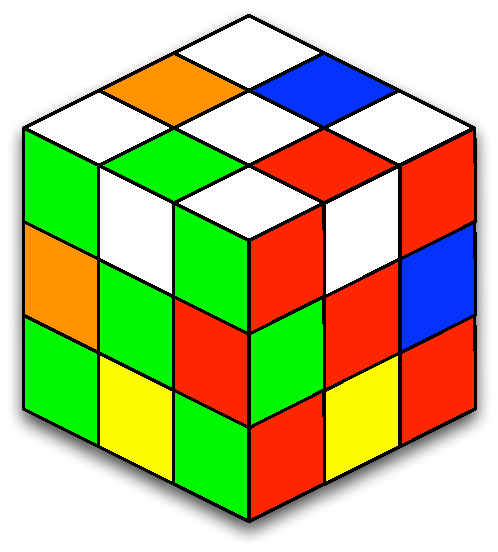
\includegraphics[scale = 0.7]{input/pics/superflip.pdf}
	\caption{\myCaption{The superflip: every edge is flipped. The optimal solution to this position is 20 twists.}}
	\label{fig:superflip}
\end{figure}





\myTail{The current upper bound is proven to be 22 twists by Thomas Rokicki using a modified version of Kociemba's optimal solver, solving a set at a time rather than just a single \rubik{}. The upper bound may be lowered in the future, it is however currently difficult due to how much CPU time is needed. The current lower bound has been proven to be 20 twists}